\documentclass[12pt,fullpage,letterpaper]{article}

\newenvironment{proof}{\noindent{\bf Proof:}}{\qed\bigskip}

\newtheorem{theorem}{Theorem}
\newtheorem{corollary}{Corollary}
\newtheorem{lemma}{Lemma} 
\newtheorem{claim}{Claim}
\newtheorem{fact}{Fact}
\newtheorem{definition}{Definition}
\newtheorem{assumption}{Assumption}
\newtheorem{observation}{Observation}
\newtheorem{example}{Example}
\newcommand{\qed}{\rule{7pt}{7pt}}

\newcommand{\assignment}[4]{
\thispagestyle{plain} 
\newpage
\setcounter{page}{1}
\noindent
\begin{center}
\framebox{ \vbox{ \hbox to 6.28in
{\bf CS446: Machine Learning \hfill #1}
\vspace{4mm}
\hbox to 6.28in
{\hspace{2.5in}\large\mbox{Problem Set #2}}
\vspace{4mm}
\hbox to 6.28in
{{\it Handed Out: #3 \hfill Due: #4}}
}}
\end{center}
}


\newcommand{\handout}[3]{
\thispagestyle{plain} 
\newpage
\setcounter{page}{1}
\noindent
\begin{center}
\framebox{ \vbox{ \hbox to 6.28in
{\bf CS446: Machine Learning \hfill #1}
\vspace{4mm}
\hbox to 6.28in
{\hspace{2.5in}\large\mbox{#2}}
\vspace{4mm}
\hbox to 6.28in
{{\it Handed Out: #3 \hfill Name (NetID): \rule[-2pt]{4cm}{0.1pt} }}
}}
\end{center}
}


\newcommand{\assgsoln}[4]{
\thispagestyle{plain} 
\newpage
\setcounter{page}{1}
\noindent
\begin{center}
\framebox{ \vbox{ \hbox to 6.28in
{\bf CS446: Machine Learning \hfill #1}
\vspace{4mm}
\hbox to 6.28in
{\hspace{2.5in}\large\mbox{Problem Set #2 Solutions}}
\vspace{4mm}
\hbox to 6.28in
{{\it Handed Out: #3 \hfill Handed In: #4}}
}}
\end{center}
}


\newcommand{\solution}[4]{
\thispagestyle{plain} 
\newpage
\setcounter{page}{1}
\noindent
\begin{center}
\framebox{ \vbox{ \hbox to 6.28in
{\bf CS446: Machine Learning \hfill #4}
\vspace{4mm}
\hbox to 6.28in
{\hspace{2.5in}\large\mbox{Problem Set #3}}
\vspace{4mm}
\hbox to 6.28in
{#1 \hfill {\it Handed In: #2}}
}}
\end{center}
\markright{#1}
}


\newenvironment{algorithm}
{\begin{center}
\begin{tabular}{|l|}
\hline
\begin{minipage}{1in}
\begin{tabbing}
\quad\=\qquad\=\qquad\=\qquad\=\qquad\=\qquad\=\qquad\=\kill}
{\end{tabbing}
\end{minipage} \\
\hline
\end{tabular}
\end{center}}

\def\Comment#1{\textsf{\textsl{$\langle\!\langle$#1\/$\rangle\!\rangle$}}}


\usepackage{amsmath}
\usepackage{algorithm}% http://ctan.org/pkg/algorithm
\usepackage{algpseudocode}% http://ctan.org/pkg/algorithmicx
\usepackage{graphicx}
\usepackage{listings}
\graphicspath{ {.} }

\DeclareMathOperator{\proj}{proj}
\newcommand{\vctproj}[2][]{\proj_{\vec{#1}}\vec{#2}}

\oddsidemargin 0in
\evensidemargin 0in
\textwidth 6.5in
\topmargin -0.5in
\textheight 9.0in

\begin{document}

\solution{Bangqi Wang}{\today}{2}{Spring 2017}
% Fill in the above, for example, as follows:
% \solution{Joe Smith}{\today}{1}{Fall 2012}

\pagestyle{myheadings}  % Leave this command alone

\begin{enumerate}
\item[1.] Answer to problem 1
	\begin{enumerate}
	\item[a.] The root of the decision tree is the attribute that has largest information gain.\\
		\begin{table}[h]
			\centering
			\begin{tabular}[h]{|c|c|c|c|c|}
				\hline
				\texttt{Attribute} & \texttt{Value} & \texttt{Study Today = yes} & \texttt{Study Today = no} \\
				\hline
				Holiday      & yes      & 20   & 1       \\
				Holiday      & no      & 15   & 14        \\
				Exam Tomorrow      & yes      & 10       & 5        \\
				Exam Tomorrow      & no      & 25       & 10        \\
				\hline
			\end{tabular}
			\caption{The {\tt Study Pattern} data set}
			\label{tab:Balloons}
		\end{table}
		\begin{itemize}
		\item $Gain(S,a) \equiv Entropy(S)\ - \sum_{v \in Values(a)} \frac{|S_{v}|}{|S|}
Entropy(S_{v})$
		\item $Entropy(S)$:
			\begin{itemize}
			\item $Entropy(S) = -\frac{35}{50} log(\frac{35}{50}) -\frac{15}{50} log(\frac{15}{50}) \approx 0.611$
			\item $Entropy(S_{Holidy=yes}) = -\frac{20}{21} log(\frac{20}{21}) -\frac{1}{21} log(\frac{1}{21})\approx 0.191$
			\item $Entropy(S_{Holidy=no}) = -\frac{15}{29} log(\frac{15}{29}) -\frac{14}{29} log(\frac{14}{29}) \approx 0.693$
			\item $Entropy(S_{Exam=yes}) = -\frac{10}{15} log(\frac{10}{15}) -\frac{5}{15} log(\frac{5}{15}) \approx 0.637$
			\item $Entropy(S_{Exam=no}) = -\frac{25}{35} log(\frac{25}{35}) -\frac{10}{35} log(\frac{10}{35}) \approx 0.598$
			\end{itemize}
		\item $Gain(S,a)$:
			\begin{itemize}
			\item $Gain(S, Holiday) $\\$ = Entropy(S)\ - \frac{|S_{Holiday=yes}|}{|S|} Entropy(S_{Holiday=yes})\ - \frac{|S_{Holiday=no}|}{|S|} Entropy(S_{Holiday=no}) $\\$ = 0.611 - \frac{21}{50} \times 0.191 - \frac{29}{50} \times 0.693 \approx 0.129$
			\item $Gain(S, Exam) $\\$ = Entropy(S)\ - \frac{|S_{Exam=yes}|}{|S|} Entropy(S_{Exam=yes})\ - \frac{|S_{Exam=no}|}{|S|} Entropy(S_{Exam=no}) $\\$ = 0.611 - \frac{15}{50} \times 0.637 - \frac{35}{50} \times 0.598 \approx 0.0013$
			\end{itemize}
		\item \textbf{Holiday} is the attribute that will be the root of the decision tree because it has largest information gain.\\
		\end{itemize}
	\item[b.]
		\begin{verbatim}
			if Color = Blue:
			    if Size = Small:
			        Inflated = F
			    if Size = Large:
			        if Act = Stretch:
			            if Age = Adult:
			                Inflated = F
			            if Age = Child:
			                Inflated = T
			        if Act = Dip:
			            Inflated = T
			if Color = Red:
			    if Size = Small:
			        if Act = Stretch:
			            if Age = Adult:
			                Inflated = F
			            if Age = Child:
			                Inflated = T
			        if Act = Dip:
			            Inflated = T
			    if Size = Large:
			        if Act = Stretch:
			            if Age = Adult:
			                Inflated = F
			            if Age = Child:
			                Inflated = T
			        if Act = Dip:
			            Inflated = T

		\end{verbatim}
	\item[c.] Finding the optimal decision tree is NP-Complete. The ID3 algorithm are based on greedy heuristics that split the attribute based on locally optimal decisions, information gain. Therefore, ID3 cannot guanrantee a globally optimal decision tree because there is no backtracking after greedily selecting locally optimal decisions.\\
	\end{enumerate}
\item[2.] Answer to problem 2
	\begin{enumerate}
	\item[a.] FeatureGenerator.java: extract 10 features from firstname and lastname.\\ \\
		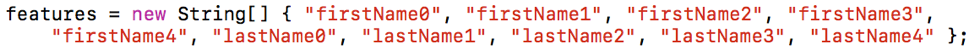
\includegraphics[width=15cm]{Picture1} \\
		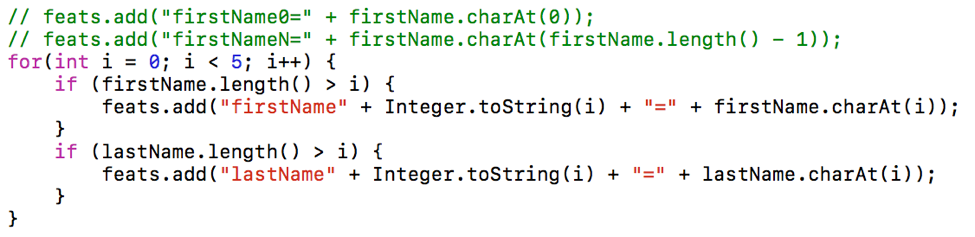
\includegraphics[width=15cm]{Picture2} \\
		For question a, I generated ten feature types. the features \textit{firstName0-4} stand for the first five characters in first name, and features \textit{lastName0-4} stand for the first five characters in last name. 
	\end{enumerate}
	\item[b.] 
		\begin{itemize}
		\item The table below shows the accuracy of algorithms in descending order.\\
			\begin{table}[h]
				\centering
				\begin{tabular}[h]{|c|c|c|c|c|c|c|c|c|}
					\hline
					\texttt{Algorithm} & \texttt{fold1} & \texttt{fold2} & \texttt{fold3} & \texttt{fold4} & \texttt{fold5} & \texttt{$p_A$} & \texttt{$\sigma$} & \texttt{$99\%$ interval} \\
					\hline
					$DT$      & 72.31\%    & 70.18\%    & 76.09\%    & 74.24\%    & 68.33\%    & 72.23\%    & 0.028    & [64.25\%, 80.21\%]\\
					$Stumps$  & 76.92\%    & 64.91\%    & 69.57\%    & 77.27\%    & 68.33\%    & 71.40\%    & 0.049    & [57.30\%, 85.50\%]\\
					$DT_8$    & 73.85\%    & 71.93\%    & 63.04\%    & 71.21\%    & 68.33\%    & 69.67\%    & 0.038    & [58.84\%, 80.50\%]\\
					$DT_4$    & 60.00\%    & 68.42\%    & 58.70\%    & 72.73\%    & 68.33\%    & 65.64\%    & 0.054    & [50.12\%, 81.16\%]\\
					$SGD$     & 67.69\%    & 71.93\%    & 56.52\%    & 75.76\%    & 51.67\%    & 64.65\%    & 0.092    & [38.31\%, 91.11\%]\\
					\hline
				\end{tabular}
				\caption{The {\tt Accuracy} for five algorithms}
				\label{tab:Balloons}
			\end{table}
		\item Calculating $99\%$ confidence intervals:\\
			\begin{eqnarray}
			I && = \: [p_A - \frac{t \times \sigma}{\sqrt{N}}, \: p_A + \frac{t \times \sigma}{\sqrt{N}}], \: t_{0.995} = 2.576\\
			I_{DT} && = \: 72.23\% \pm \frac{2.576 \times 0.028}{\sqrt{5}} \: = \: [64.25\%, 80.21\%] \\
			I_{Stumps} && = \: 71.40\% \pm \frac{2.576 \times 0.049}{\sqrt{5}} \: = \: [57.30\%, 85.50\%] \\
			I_{DT_8} && = \: 79.67\% \pm \frac{2.576 \times 0.038}{\sqrt{5}} \: = \: [58.84\%, 80.50\%] \\
			I_{DT_4} && = \: 65.64\% \pm \frac{2.576 \times 0.054}{\sqrt{5}} \: = \: [50.12\%, 81.16\%] \\
			I_{SGD} && = \: 64.65\% \pm \frac{2.576 \times 0.092}{\sqrt{5}} \: = \: [38.31\%, 91.11\%]
			\end{eqnarray}
		\item To show if the difference between the two consecutive algorithm's performance is or is not statistically significant:
			\begin{itemize}
			\item $DT \rightarrow Stumps$: No
			\item $Stumps \rightarrow DT_8$: No 
			\item $DT_8 \rightarrow DT_4$: No
			\item $DT_4 \rightarrow SGD$: No \\
			\end{itemize}
		\item \textbf{Implement}:
			\begin{itemize}
			\item \textbf{Decision Tree}:\\
			The implementation of decision tree is in folder $/bwang34-hw2/data/decision-trees/src/$. The tree structure is in $Id3.java$ and the decision tree classifier is in $WekaTester.java$. \\
			\item \textbf{SGD}:\\
			The implementation of SGD is in the same folder. The SGD structure is in $Gradient.java$. This SGD structure is similar to Id3 structure in $Classifier$ class. The classifier is also in $WekaTester.java$ and has similar usage as $Id3$. \\
			\item \textbf{Decision Stumps}:\\
			The implementation of Decision Stumps is also in the same folder. The strucutre is in $WekaTester.java$. I first construct $100$ decision tree with depth 4, and then use the labels as new features. Finally, I run $SGD$ classifier on those new features with five-fold cross validation. \\
			\end{itemize}
		\item \textbf{Parameter Tuning}:
			\begin{table}[h]
				\centering
				\begin{tabular}[h]{|c|c|c|c|c|c|c|}
					\hline
					\texttt{(rate,threshold)} & \texttt{fold1} & \texttt{fold2} & \texttt{fold3} & \texttt{fold4} & \texttt{fold5} & \texttt{$p_A$}\\
					\hline
					$(0.001, 20)$     & 61.54\%    & 68.42\%    & 65.22\%    & 77.27\%    & 65.00\%    & 67.49\% \\
					$(0.0001, 20)$    & 70.77\%    & 63.16\%    & 60.87\%    & 75.76\%    & 66.67\%    & 67.45\% \\
					$(0.00001, 20)$   & 75.38\%    & 64.91\%    & 63.04\%    & 78.79\%    & 71.67\%    & 70.77\% \\
					$(0.00001, 50)$   & 64.62\%    & 70.18\%    & 67.39\%    & 84.85\%    & 68.33\%    & 71.01\% \\
					$(0.00001, 100)$  & 76.92\%    & 64.91\%    & 69.57\%    & 77.27\%    & 68.33\%    & 71.40\% \\
					\hline
				\end{tabular}
				\caption{The {\tt Accuracy} for Decision Stumps with Depth 4 Decision Tree }
				\label{tab:Balloons}
			\end{table}
			\begin{itemize}
				\item The final learning rate is 0.00001, and the threshold is 100.\\
			\end{itemize}
		\item \textbf{Conclusion}:
			\begin{itemize}
			\item Decision tree with more depth is more accurarte.
			\item SGD is unstable with large fluctuation. The confidence interval is wide.
			\item Decision Stumps is much more acurate than decision tree with same depth and SGD. Decision Stumps constructed by decision tree with depth 4 is much acurate than decision tree with depth 4 and 8.
			\item High learning rate might cause earlier saturation so the accuracy is lower.
			\item High thredhold can increase the accuracy for Decision Stumps because it avoids the overfitting of each decision tree.\\
			\end{itemize}
		\item \textbf{Code}:\\
			Folder: $/bwang34-hw2/data/decision-trees/src/$\\
			Files:
				\begin{itemize}
					\item SGD - $Gradient.java$
					\item Decision Stumps - $WekaTester.java$
					\item Decision Tree - $Id3.java$
					\item Feature Generator - $FeatureGenerator.java$
				\end{itemize}
			.\\\\
		\item \textbf{Tree Display}:
			\begin{itemize}
				\item \textbf{Decision Tree}: \\
					\begin{verbatim}
					==================================================
					ID3, unlimited, fold3

					ID3

					lastName0=m = 1
					|  firstName2=e = 1: +
					|  firstName2=e = 0
					|  |  lastName1=o = 1: +
					|  |  lastName1=o = 0
					|  |  |  firstName0=p = 1: -
					|  |  |  firstName0=p = 0
					|  |  |  |  firstName0=r = 1: -
					|  |  |  |  firstName0=r = 0
					|  |  |  |  |  firstName0=y = 1: -
					|  |  |  |  |  firstName0=y = 0
					|  |  |  |  |  |  firstName1=u = 1: -
					|  |  |  |  |  |  firstName1=u = 0
					|  |  |  |  |  |  |  lastName3=a = 1
					|  |  |  |  |  |  |  |  firstName3=r = 1: +
					|  |  |  |  |  |  |  |  firstName3=r = 0: -
					|  |  |  |  |  |  |  lastName3=a = 0: +
					lastName0=m = 0
					|  lastName1=l = 1
					|  |  firstName0=d = 1: -
					|  |  firstName0=d = 0: +
					|  lastName1=l = 0
					|  |  lastName2=l = 1
					|  |  |  firstName2=r = 1: -
					|  |  |  firstName2=r = 0
					|  |  |  |  lastName4=n = 1: -
					|  |  |  |  lastName4=n = 0
					|  |  |  |  |  firstName2=h = 1: -
					|  |  |  |  |  firstName2=h = 0: +
					|  |  lastName2=l = 0
					|  |  |  lastName2=o = 1
					|  |  |  |  firstName0=b = 1: -
					|  |  |  |  firstName0=b = 0: +
					|  |  |  lastName2=o = 0
					|  |  |  |  firstName3=f = 1: +
					|  |  |  |  firstName3=f = 0
					|  |  |  |  |  lastName4=l = 1
					|  |  |  |  |  |  firstName2=h = 1: -
					|  |  |  |  |  |  firstName2=h = 0
					|  |  |  |  |  |  |  lastName0=l = 1: -
					|  |  |  |  |  |  |  lastName0=l = 0
					|  |  |  |  |  |  |  |  lastName0=q = 1: -
					|  |  |  |  |  |  |  |  lastName0=q = 0: +
					|  |  |  |  |  lastName4=l = 0
					|  |  |  |  |  |  firstName1=o = 1
					|  |  |  |  |  |  |  lastName0=f = 1: -
					|  |  |  |  |  |  |  lastName0=f = 0
					|  |  |  |  |  |  |  |  firstName2=e = 1: -
					|  |  |  |  |  |  |  |  firstName2=e = 0
					|  |  |  |  |  |  |  |  |  firstName3=a = 1
					|  |  |  |  |  |  |  |  |  |  lastName0=h = 1: +
					|  |  |  |  |  |  |  |  |  |  lastName0=h = 0: -
					|  |  |  |  |  |  |  |  |  firstName3=a = 0
					|  |  |  |  |  |  |  |  |  |  firstName2=n = 1: +
					|  |  |  |  |  |  |  |  |  |  firstName2=n = 0
					|  |  |  |  |  |  |  |  |  |  |  lastName2=n = 1: +
					|  |  |  |  |  |  |  |  |  |  |  lastName2=n = 0
					|  |  |  |  |  |  |  |  |  |  |  |  lastName1=a = 1: -
					|  |  |  |  |  |  |  |  |  |  |  |  lastName1=a = 0
					|  |  |  |  |  |  |  |  |  |  |  |  |  firstName3=g = 1: -
					|  |  |  |  |  |  |  |  |  |  |  |  |  firstName3=g = 0: +
					|  |  |  |  |  |  firstName1=o = 0
					|  |  |  |  |  |  |  lastName0=l = 1
					|  |  |  |  |  |  |  |  firstName1=a = 1
					|  |  |  |  |  |  |  |  |  firstName0=d = 1: +
					|  |  |  |  |  |  |  |  |  firstName0=d = 0: -
					|  |  |  |  |  |  |  |  firstName1=a = 0: +
					|  |  |  |  |  |  |  lastName0=l = 0
					|  |  |  |  |  |  |  |  lastName3=m = 1
					|  |  |  |  |  |  |  |  |  firstName2=r = 1: -
					|  |  |  |  |  |  |  |  |  firstName2=r = 0: +
					|  |  |  |  |  |  |  |  lastName3=m = 0
					|  |  |  |  |  |  |  |  |  firstName1=e = 1
					|  |  |  |  |  |  |  |  |  |  firstName2=n = 1: +
					|  |  |  |  |  |  |  |  |  |  firstName2=n = 0
					|  |  |  |  |  |  |  |  |  |  |  firstName2=o = 1
					|  |  |  |  |  |  |  |  |  |  |  |  lastName0=b = 1: -
					|  |  |  |  |  |  |  |  |  |  |  |  lastName0=b = 0: +
					|  |  |  |  |  |  |  |  |  |  |  firstName2=o = 0
					|  |  |  |  |  |  |  |  |  |  |  |  lastName2=r = 1
					|  |  |  |  |  |  |  |  |  |  |  |  |  firstName0=m = 1: -
					|  |  |  |  |  |  |  |  |  |  |  |  |  firstName0=m = 0: +
					|  |  |  |  |  |  |  |  |  |  |  |  lastName2=r = 0: -
					|  |  |  |  |  |  |  |  |  firstName1=e = 0
					|  |  |  |  |  |  |  |  |  |  firstName0=t = 1
					|  |  |  |  |  |  |  |  |  |  |  lastName4=e = 1: -
					|  |  |  |  |  |  |  |  |  |  |  lastName4=e = 0
					|  |  |  |  |  |  |  |  |  |  |  |  lastName0=s = 1: -
					|  |  |  |  |  |  |  |  |  |  |  |  lastName0=s = 0: +
					|  |  |  |  |  |  |  |  |  |  firstName0=t = 0
					|  |  |  |  |  |  |  |  |  |  |  firstName3=o = 1
					|  |  |  |  |  |  |  |  |  |  |  |  firstName0=a = 1: +
					|  |  |  |  |  |  |  |  |  |  |  |  firstName0=a = 0
					|  |  |  |  |  |  |  |  |  |  |  |  |  firstName0=m = 1: +
					|  |  |  |  |  |  |  |  |  |  |  |  |  firstName0=m = 0: -
					|  |  |  |  |  |  |  |  |  |  |  firstName3=o = 0
					|  |  |  |  |  |  |  |  |  |  |  |  firstName4=o = 1
					|  |  |  |  |  |  |  |  |  |  |  |  |  firstName0=s = 1: -
					|  |  |  |  |  |  |  |  |  |  |  |  |  firstName0=s = 0: +
					|  |  |  |  |  |  |  |  |  |  |  |  firstName4=o = 0
					|  |  |  |  |  |  |  |  |  |  |  |  |  lastName0=s = 1
					|  |  |  |  |  |  |  |  |  |  |  |  |  |  firstName0=d = 1: +
					|  |  |  |  |  |  |  |  |  |  |  |  |  |  firstName0=d = 0
					|  |  |  |  |  |  |  |  |  |  |  |  |  |  |  lastName4=h = 1
					|  |  |  |  |  |  |  |  |  |  |  |  |  |  |  |  firstName0=s = 1: -
					|  |  |  |  |  |  |  |  |  |  |  |  |  |  |  |  firstName0=s = 0: +
					|  |  |  |  |  |  |  |  |  |  |  |  |  |  |  lastName4=h = 0: -
					|  |  |  |  |  |  |  |  |  |  |  |  |  lastName0=s = 0
					|  |  |  |  |  |  |  |  |  |  |  |  |  |  lastName3=l = 1
					|  |  |  |  |  |  |  |  |  |  |  |  |  |  |  firstName0=d = 1: -
					|  |  |  |  |  |  |  |  |  |  |  |  |  |  |  firstName0=d = 0: +
					|  |  |  |  |  |  |  |  |  |  |  |  |  |  lastName3=l = 0: -


					Correctly Classified Instances          35               76.087  %
					Incorrectly Classified Instances        11               23.913  %
					Kappa statistic                          0.5199
					Mean absolute error                      0.2391
					Root mean squared error                  0.489
					Relative absolute error                 48.1752 %
					Root relative squared error             98.1732 %
					Total Number of Instances               46
					\end{verbatim}
					.\\\\
				\item \textbf{Decision Stumps}: \\
					\begin{verbatim}
					Decision Stumps, fold4

					cs446.homework2.Gradient@681a9515


					Correctly Classified Instances          51               77.2727 %
					Incorrectly Classified Instances        15               22.7273 %
					Kappa statistic                          0.5326
					Mean absolute error                      0.2273
					Root mean squared error                  0.4767
					Relative absolute error                 46.9613 %
					Root relative squared error             96.961  %
					Total Number of Instances               66
					\end{verbatim}
					.\\\\
				\item \textbf{Decision Tree - 8}: \\
					\begin{verbatim}
					==================================================
					ID3, depth 8, fold1

					ID3

					firstName3=f = 1: +
					firstName3=f = 0
					|  lastName0=c = 1: -
					|  lastName0=c = 0
					|  |  lastName4=l = 1
					|  |  |  lastName0=q = 1: -
					|  |  |  lastName0=q = 0: +
					|  |  lastName4=l = 0
					|  |  |  firstName0=r = 1
					|  |  |  |  firstName1=o = 1: +
					|  |  |  |  firstName1=o = 0
					|  |  |  |  |  firstName1=a = 1: +
					|  |  |  |  |  firstName1=a = 0
					|  |  |  |  |  |  firstName1=e = 1: +
					|  |  |  |  |  |  firstName1=e = 0: -
					|  |  |  firstName0=r = 0
					|  |  |  |  lastName0=m = 1
					|  |  |  |  |  firstName2=n = 1: -
					|  |  |  |  |  firstName2=n = 0
					|  |  |  |  |  |  firstName0=p = 1: -
					|  |  |  |  |  |  firstName0=p = 0
					|  |  |  |  |  |  |  lastName2=t = 1
					|  |  |  |  |  |  |  |  firstName0=t = 1: +
					|  |  |  |  |  |  |  |  firstName0=t = 0: -
					|  |  |  |  |  |  |  lastName2=t = 0: +
					|  |  |  |  lastName0=m = 0
					|  |  |  |  |  lastName0=l = 1
					|  |  |  |  |  |  firstName1=a = 1
					|  |  |  |  |  |  |  firstName0=d = 1: +
					|  |  |  |  |  |  |  firstName0=d = 0: -
					|  |  |  |  |  |  firstName1=a = 0: +
					|  |  |  |  |  lastName0=l = 0
					|  |  |  |  |  |  lastName3=m = 1
					|  |  |  |  |  |  |  firstName2=r = 1: -
					|  |  |  |  |  |  |  firstName2=r = 0: +
					|  |  |  |  |  |  lastName3=m = 0
					|  |  |  |  |  |  |  lastName2=l = 1
					|  |  |  |  |  |  |  |  firstName2=r = 1: -
					|  |  |  |  |  |  |  |  firstName2=r = 0: +
					|  |  |  |  |  |  |  lastName2=l = 0
					|  |  |  |  |  |  |  |  lastName3=l = 1: +
					|  |  |  |  |  |  |  |  lastName3=l = 0: -


					Correctly Classified Instances          48               73.8462 %
					Incorrectly Classified Instances        17               26.1538 %
					Kappa statistic                          0.4785
					Mean absolute error                      0.3371
					Root mean squared error                  0.4722
					Relative absolute error                 67.4285 %
					Root relative squared error             94.4514 %
					Total Number of Instances               65
					\end{verbatim}
					.\\\\
				\item \textbf{Decision Tree - 4}: \\
					\begin{verbatim}
					==================================================
					ID3, depth 4, fold4

					ID3

					lastName2=l = 1
					|  firstName2=r = 1: -
					|  firstName2=r = 0
					|  |  firstName2=m = 1: -
					|  |  firstName2=m = 0: +
					lastName2=l = 0
					|  lastName2=o = 1
					|  |  firstName0=d = 1: -
					|  |  firstName0=d = 0
					|  |  |  firstName2=l = 1: -
					|  |  |  firstName2=l = 0: +
					|  lastName2=o = 0
					|  |  firstName3=f = 1: +
					|  |  firstName3=f = 0
					|  |  |  lastName0=m = 1
					|  |  |  |  firstName0=n = 1: -
					|  |  |  |  firstName0=n = 0: +
					|  |  |  lastName0=m = 0
					|  |  |  |  lastName1=l = 1: +
					|  |  |  |  lastName1=l = 0: -


					Correctly Classified Instances          48               72.7273 %
					Incorrectly Classified Instances        18               27.2727 %
					Kappa statistic                          0.409
					Mean absolute error                      0.3812
					Root mean squared error                  0.4582
					Relative absolute error                 78.7652 %
					Root relative squared error             93.1911 %
					Total Number of Instances               66
					\end{verbatim}
					.\\\\
				\item \textbf{SGD}: \\
					\begin{verbatim}
					==================================================
					SGD, fold4

					cs446.homework2.Gradient@6b884d57


					Correctly Classified Instances          50               75.7576 %
					Incorrectly Classified Instances        16               24.2424 %
					Kappa statistic                          0.5152
					Mean absolute error                      0.2424
					Root mean squared error                  0.4924
					Relative absolute error                 50.0921 %
					Root relative squared error            100.1409 %
					Total Number of Instances               66
					\end{verbatim}
					.\\\\
			\end{itemize}
		\end{itemize}
\end{enumerate}

\end{document}

